%
% Der Satz von Green
%
\section{Der Satz von Green
\label{buch:green:section:green}}
\kopfrechts{Der Satz von Green}
Der Hauptsatz der Infinitesimalrechnung besagt, dass man das Integral
einer Ableitung aus den Werten am Intervallende erhalten kann.
Diese Idee wurde bereits in Kapitel~\ref{chapter:kurvenintegral} auf
das Integral einer 1-Form verallgemeinert.
Das Integral eines Differentials $df$ entlang einer Kurve ist durch
die Werte der Funktion $f$ in den Endpunkten gegeben.
Im vorliegenden Abschnitt soll eine ähnliche Ausssage für Integrale
von 2-Formen über zweidimensionale Gebiete abgeleitet werden.
Der Satz von Green stellt einen Zusammenhang zwischen dem Integral
gewisser Ableitungen über das Innere eines Gebietes und den Werten
auf dem Rand dar.
Es soll gezeigt werden, dass die Ableitung eine natürlich Erweiterung
des Differentials $df$ einer Funktion ist.
In späteren Kapiteln soll dies dann zum allgemeinen Satz von Stokes
verallgemeinert werden.
Die auf diese Weise aus dem Differential $d$ erhaltenen
Differentialoperatoren sind die natürlichen Operatoren, die für
eine koordinatenfreie Formulierung von Naturgesetzen geeignet sind.
So wie wir das Differential bereits als Gradient einer Funktion
interpretiert haben, soll die Ableitung von 1- und 2-Formen später
als die in den Anwendungen weit verbreitet Operation der Rotation
und der Divergenz erkannt werden.

%
% Zerlegung in Koordinatengebiete
%
\subsection{Zerlegung in Koordinatengebiete
\label{buch:green:satzvongreen:subsection:zerlegung}}
In Abschnitt~\ref{buch:kurvenintegral:section:zerlegung} wurde gezeigt,
wie sich ein Integral einer $1$-Form über eine Kurve mit Hilfe einer
Zerlegung der Einheit durch endlich viele beliebig oft differenzierbare
Funktionen $g_i$ in eine endlich Summe
\[
\int_{\gamma} \alpha = \sum_i \int_{\gamma} g_i\alpha_i
\]
von Integralen von differenzierbaren 1-Formen zerlegen, wobei der
Träger von $g_i$ immer in einem Koordinatengebiet enthalten war.
Diese Vorgehensweise lässt sich auch auf zweidimensionale Gebiete
übertragen.

Im folgenden betrachten wir nur kompakte Mannigfaltigketen, da nicht
kompakte Mannigfaltigkeiten ohnehin zu nicht definierten Integralen
führen können.

Ein Quader in $\mathbb{R}^n$ ist ein kartesisches Produkt
\[
Q
=
(a_1,b_1)
\times\dots\times
(a_n,b_n)
=
\{
(x^1,\dots,x^n)\in\mathbb{R}^n
\mid
a_i < x^i < b_i
\;\forall i=1,\dots,n
\}.
\]
Die Funktionen
\[
g_Q(x)
=
g_{a_1,b_1}(x^1)\dots g_{a_n,b_n}(x^n)
\]
sind beliebig oft differenzierbare Funktionen, die genau im Quader
$Q$ von $0$ verschieden sind.

Eine beschränkte offene Menge $U\subset\mathbb{R}^n$ kann, wie in
Abbildung~\ref{XXX} am zweidimensionalen Beispiel gezeigt,
von innen durch Quader approximiert werden.
Ist $F\subset U$ eine abgeschlossene Teilmenge, dann ist sie auch
kompakt und kann daher von endlich vielen Quadern überdeckt werden.
Durch Addition der zugehörigen Funktionen der Form $g_Q$ kann man also
eine beliebig oft differenzierbare Funktion finden, die auf $F$ von
$0$ verschieden ist und deren Träger ganz in $U$ enthalten ist.

Wir wenden diese Überlegung jetzt auf die Kartengebiete eines
Atlas $(U_\alpha)_{\alpha\in I}$ einer kompakten Mannigfaltigkeit an.
Da die Mannigfaltigkeit kompakt ist, dürfen wir sogar annehmen, dass
der Atlas aus nur endlich vielen Karten besteht.
In jedem Kartengebiet wählen wir jetzt eine Vereinigung $V_\alpha$
von offenen Quadern so, dass auch die Mengen $V_\alpha$ die ganze
Mannigfaltigkeit überdecken.

\begin{satz}
Sei $(U_\alpha,\varphi_\alpha)$ eine endliche Familie von Karten,
die eine kompakte Mannigfaltigkeit überdecken.
Dann gibt es Teilmengen $V_\alpha\subset U_\alpha$, die endliche
Vereingungen von Quadern sind derart, dass die eingeschränkten Karten
$(V_\alpha,\varphi_\alpha\mathstrut_{|V_\alpha})$ ebenfalls einen Atlas
bilden.
\end{satz}

\begin{proof}
Zu jedem $\alpha$ und Punkt $x\in U_\alpha$ gibt es einen offenen
Quader $Q_{x,\alpha}$, der $x$ enthält und in $U_\alpha$ enthalten
ist: $x\in Q_{x,\alpha}\subset U_\alpha$.
Die Vereinigung der $Q_{x,\alpha}$ ist eine Überdeckung der
Mannigfaltigkeit.
Da die Mannigfaltigkeit $M$ kompakt ist, gibt es auch eine endliche 
Teilmenge, die bereits $M$ überdeckt.
Bildet man für jedes $\alpha$ die Mengen $V_\alpha$ aus den Quadern
$Q_{x,\alpha}$, dann ist $V_\alpha$ eine Überdeckung der Mannigfaltigkeit
der verlangten Art.
\end{proof}

In einer Überdeckung einer Mannigfaltigkeit durch die Vereinigungen
$V_\alpha$ von Quadern kann man eine Menge von beliebig oft
differenzierbaren Funktionen
$g_\alpha$ ableiten, die genau auf $V_\alpha$ von $0$ verschieden
sind.
Da die $V_\alpha$ eine Überdeckung bilden, ist die Summe
\[
G(x) = \sum_{\alpha} g_\alpha(x)
\]
auf der ganzen Mannigfaltigkeit von $0$ verschieden und kann dazu
benutzt werden, die Funktionen $g_\alpha$ auf
\[
h_\alpha(x) = \frac{1}{G(x)}\,g_\alpha(x)
\]
zu normieren, die eine Zerlegung der Einheit bilden.

Auf einem Kartengebiet einer zweidimensionalen Mannigfaltigkeit
ist bereits bekannt, wie eine 2-Form integriert werden kann.
Mit einer Zerlegung der Einheit, wie sie oben konstruiert worden ist,
lässt sich jetzt das Integral einer beliebigen 2-Form jetzt über
die ganze Mannigfaltigkeit erstrecken.
Dazu schreibt man
\[
\int_M \alpha
=
\int_M \sum_{\alpha}h_\alpha\,\alpha
=
\int_{V_\alpha} h_\alpha\,\alpha.
\]
Dies ist möglich, weil $h_\alpha\,\alpha$ nur innerhalb von $V_\alpha$
von $0$ verschieden ist.
Die 2-Form $h_\alpha\,\alpha$ kann im Kartengebiet durch die
Komponenten dargestellt und integriert werden.

%
% Interal in einem Koordinatengebiet
%
\subsection{Integral in einem Koordinatengebiet}
Dank der Zerlegung eines Integrals gemäss
Abschnitt~\ref{buch:green:satzvongreen:subsection:zerlegung}
muss in diesem Abschnitt nur noch das Integral einer 2-Form in
einem Koordinatengebiet berechnet werden.
Wir nehmen daher an, dass die 2-Form durch
\[
\omega
=
a_{ik}(x)\,dx^i\wedge dx^k
\]
gegeben ist, wobei die Koeffizienten $a_{ik}(x)$ ausserhalb
von $V_\alpha$ verschwindet.

%
% Integral über ein Gebiet ohne Rand
%
\subsubsection{Integral über ein Gebiet ohne Rand}
In den Koordinaten der Karte wird das Integral der 2-Form $\omega$
durch
\begin{equation}
\int_M \omega
=
\int_{\varphi_\alpha(V_\alpha)}
a_{ik}(x)\, v(x)
\,dx^1\,dx^2
\label{buch:green:green:eqn:koordinatenform}
\end{equation}
gegeben.
% XXX was ist v(x)
Da $\omega$ ausserhalb von $V_\alpha$ verschwindet, können wir $\omega$
durch 0 auf ganz $\mathbb{R}^2$ ausdehnen und integrieren.

Für das im Satz von Green angestrebte Resultat berechnen wird das
Integral einer 2-Form der Form
\[
\frac{\partial f_i}{\partial x^k}(x)\, dx^i \wedge dx^k,
\]
wobei $i\ne k$ ist.
Einsetzen der Definition in
\eqref{buch:green:green:eqn:koordinatenform}
ergibt das Integral
\begin{align*}
\int_M\omega
&=
\int\hspace*{-2mm}\int_{\varphi_\alpha(V_\alpha)}
\frac{\partial f_i}{\partial x^k}(x)
\, dx^i \, dx^k.
\intertext{Nach dem Satz von Fubini können die Integrale über die
Variablen unabhängig voneinander durchgeführt werden.
Wir schreiben daher}
&=
\int_{-\infty}^{\infty}
\int_{-\infty}^{\infty}
\frac{\partial f_i}{\partial x^k}(x)
\,dx^k
\,dx^i.
\intertext{Das innere Integral kann ausgeführt werden und ergibt}
&=
\int_{-\infty}^{\infty}
\biggl[f_i(x)\biggr]_{-\infty}^{\infty}
\,dx^i.
\intertext{Da $f_i(x)$ ausserhalb des Gebietes $\varphi_\alpha(V_\alpha)$
verschwindet, ist der Integrand $0$ und damit auch}
\int_{V_\alpha} \omega
&=
0.
\end{align*}
Für eine 2-Form, deren Koeffizienten eine Ableitung sind, verschwindet
also das Integral über ein Gebiet ohne Rand.

%
% Der Rand eines Gebietes
%
\subsubsection{Der Rand eines Gebietes}
%
% fig-randkarten.tex
%
% (c) 2025 Prof Dr Andreas Müller
%
\begin{figure}
\centering
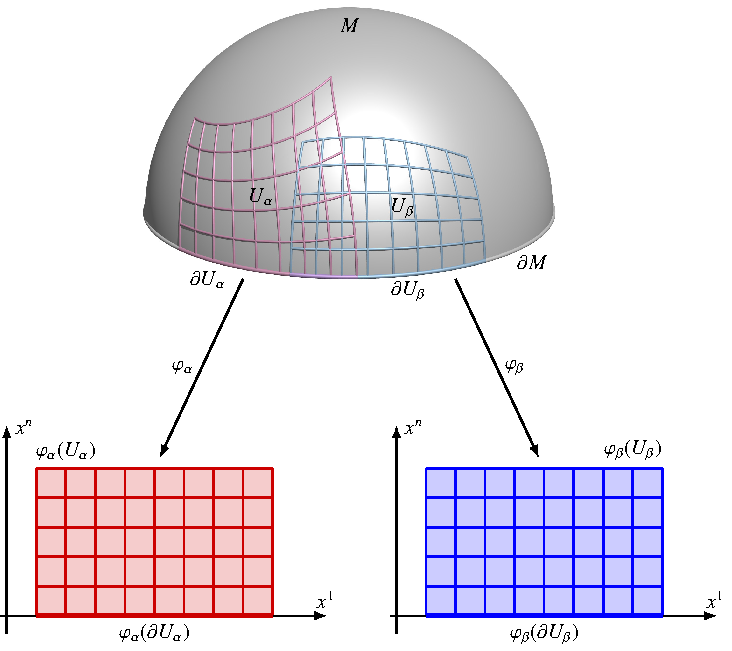
\includegraphics{chapters/040-green/images/randkarten.pdf}
\caption{Eine Mannigfaltigkeit mit Rand hat Karten, die eine offene
Teilmenge von $\{x^n=0\}$ als Rand enthalten.
Kartenwechsel sind beliebig oft differenzierbare Abbildungen, die
Randteile in Randteile abbilden (ausgezogene Linien entlang der
Hyperebene $\{x^n=0\}$).
\label{buch:green:green:fig:randkarten}}
\end{figure}

Der Wert des Kurvenintegrals der 1-Form $df$ entlang einer
Kurve zwischen zwei Punkten $A$ und $B$ in einer $n$-dimensionalen
Mannigfaltigkeit wird durch die Werte von $f$ in den Endpunkten
gegeben.
Das Integrationsgebiet $[a,b]$ ist nicht eine eindimensionale
Mannigfaltigkeit, da in einer solchen jeder Punkt eine Umgebung
hat, die homöomorph zu einem offenen Intervall in $\mathbb{R}$ ist.
Die beiden Endpunkt haben diese Eigenschaft nicht, sie haben eine
Umgebung, die homöomorph zum halboffenen Intervall $[0,1)$ für
den Anfangspunkt und $(-1,0]$ für den Endpunkt sind.
Man sagt, $[a,b]$ sei eine eindimensionale Mannigfaltigkeit mit
Rand.

Eine $n$-dimensionale differenzierbare Mannigfaltigkeit kann
ähnlich dadurch definiert werden, dass zusätzliche Arten von
Karten zugelassen werden.
Eine Karte $(U,\varphi)$ von $M$ ist eine Abbildung
$\varphi \colon U\to\mathbb{R}^n$, die ein Homöomorphismus
zwischen $U$ und einer offenen Teilmenge von
\[
\{
(x^1,\dots,x^n) \in\mathbb{R}^n
\mid
x^n\ge 0
\}
\]
ist.
$U$ kann also wie bisher eine offene Menge sein oder sie kann 
einen Teil der Hyperebene $x^n=0$ enthalten.
Dieser Teil $\partial U=\varphi^{-1}(\{x^n = 0\})$ ist ein Randstück und
durch weglassen der letzten Koordinate bekommen wir eine Kartenabbildung
$\varphi_{|\partial U}\colon \partial U \to \mathbb{R}^{n-1}$ für das
Randstück.
Für die Kartenwechsel wird verlangt, dass sie und die Ableitungen
beliebig oft differenzierbar sind, dass aber auch die Kartenwechsel
auf den Randteilen umkehrbare differenzierbare Abbildungen zwischen
offenen Mengen von $\mathbb{R}^{n-1}$ sein müssen.
Die Kartengebiete mit Rand müssen also einen Atlas für den Rand
der differenzierbaren Mannigfaltigkeit ergeben.

%
% Integral über den Rand
%
\subsubsection{Integral über den Rand}
%
% fig-greenrand2d.tex
%
% (c) 2025 Prof Dr Andreas Müller
%
\begin{figure}
\centering
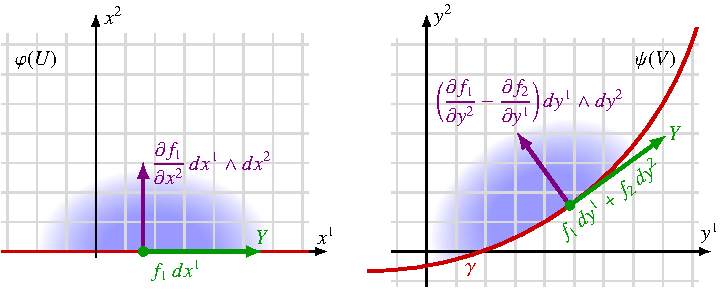
\includegraphics{chapters/040-green/images/greenrand2d.pdf}
\caption{Berechnung des Integrals einer 2-Form über ein Gebiet mit Rand.
Falls der Rand die Achse $x^2=0$ ist, ist das Integral im Wesentlichen
eine Stammfunktion des Koeffizienten.
Für gekrümmten Rand setzt sich das Integral aus den Komponenten der
Normalen zusammen.
\label{buch:green:green:fig:greenrand2d}}
\end{figure}
%
Der Satz von Green, der weiter unten formuliert wird, stellt einen
Zusammenhang eines Integrals einer 2-Form über das Gebiet und eines
Integrals einer 1-Form über den Rand her.
Dieser Zusammenhang ist in Abbildung~\ref{buch:green:green:fig:greenrand2d}
links dargestellt.
Das Integral der 
\[
\omega = \frac{\partial f_1}{\partial x_2}\,dx^1\wedge dx^2
\]
über das Kartengebiet $U$ der Karte $(U,\varphi)$ ist das Integral 
von $\omega$ gegeben durch
\begin{align*}
\int_{\varphi(U)} \omega
&=
\int_{-\infty}^{\infty}
\biggl(
\int_{0}^{\infty}
\frac{\partial f_1}{\partial x^2}(x^1,x^2)\,dx^2
\biggr)\,dx^1.
\intertext{Das $x^2$-Integral kann sofort ausgeführt werden und ist}
&=
\int_{-\infty}^{\infty}
\bigl[ f_1(x^1,x^2) \bigr]_{0}^{\infty}
\,dx^1
=
-
\int_{-\infty}^\infty
f_1(x^1,0)
\,dx^1.
\end{align*}
Das letzte Integral ist das Integral der 1-Form $f_1\,dx^1$ entlang
der $x^1$-Achse, die den Rand bildet.

Dieses Argument ist auch anwendbar, wenn der Rand gekrümmt ist,
wie dies in Abbildung~\ref{buch:green:green:fig:greenrand}
unten dargestellt ist.
%
% fig-greenrand.tex
%
% (c) 2025 Prof Dr Andreas Müller
%
\begin{figure}
\centering
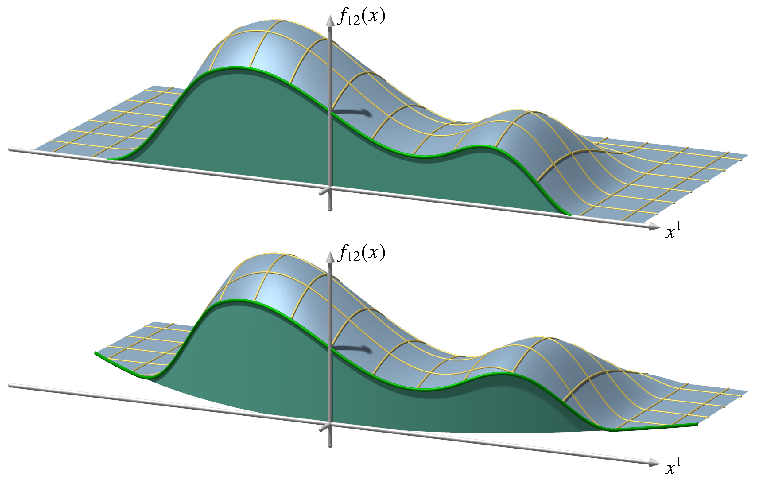
\includegraphics{chapters/040-green/images/greenrand.pdf}
\caption{Berechnung des Beitrags zum Integral einer 2-Form
$\omega = f_{12}(x)\,dx^1\wedge dx^2$, die am Rand nicht
verschwindet.
\label{buch:green:green:fig:greenrand}}
\end{figure}
%
Ist $g$ eine Funktion so, dass der Graph $x^2=g(x^1)$ den Rand
beschreibt, dann kann man das Integrationsgebiet mit den Koordinaten
\[
(y^1,y^2)
=
(x^1,x^2-g(x^1))
\]
beschreiben.
In den $(y^1,y^2)$-Koordinaten bekommt das Gebiet damit einen geraden
Rand.

Der Koordinatenwechsel für die 1-Formen ist
\begin{align*}
dy^1 &= dx^1 \\
dy^2 &= dx^2 - g'(x^1)\,dx^1.
\end{align*}
Für die daraus gebildete 2-Form gilt
\[
dy^1\wedge dy^2
=
dx^1 \wedge (dx^2 - g'(x^1)\,dx^1)
=
dx^1\wedge dx^2
-
g'(x^1)\,\underbrace{dx^1\wedge dx^1}_{\displaystyle=0}
=
dx^1\wedge dx^2.
\]

Die zu integrierende 2-Form ist
\[
\omega
=
\frac{\partial f_1}{\partial x^2}(x^1,x^2)
\,dx^1\wedge dx^2
=
\frac{\partial f_1}{\partial x^2}(y^1,y^2+g(y^1)).
\,dy^1\wedge dy^2
\]
Das Hinzufügen des nicht von $x^2$ abhängigen Terms $g(y^1)$ ändert
nichts an der Ableitung.
Das Integral der 2-Form $\omega$ wird dann
\begin{align*}
\int \omega
&=
\int_{-\infty}^{\infty}
\int_{g(x^1)}^\infty
\frac{\partial f_1}{\partial x^2}
\,dx^2
\,dx^1.
\intertext{Die Grenzen des $x^1$ Integrals sind durch den Rand des
Gebiets vorgegeben und sind im Moment nicht wichtig, da sie in den
$(y^1,y^2)$-Koordinaten ohnehin wegfallen.
Das Integral wird in $(y^1,y^2)$-Koordinaten zu}
&=
\int_{\dots}^{\dots}
\int_0^\infty
\frac{\partial f_1}{\partial x^2}(y^1,y^2+g(y^1))
\,dy^2
\,dy^1
\\
&=
\int_{-\infty}^\infty
\bigl[
f_1(y^1,y^2+g(y^1))
\bigr]_{0}^\infty
\,dy^1
\\
&=
-
\int_{-\infty}^\infty
f_1(y^1,g(y^1))
\,dy^1.
\intertext{Das letzte Integral ist das Integral der 1-Form $f_1\,dy^1$
entlang der Randkurve $\gamma(t) = (t,g(t))$:}
&=
- \int_\gamma f_1(\gamma(t))\,dt.
\end{align*}
Auch für einen gekrümmten Rand kann man also das Integral der 2-Form,
die eine Ableitung enthält, über das Gebiet durch ein Integral
einer 1-Form über den Rand ausdrücken.

%
% Integral einer 2-Form in einer Karte mit Rand
%
\subsubsection{Integral einer 2-Form in einer Karte mit Rand}
Sei jetzt $V_\alpha$ ein Randkartengebiet einer 2-dimensionalen
Mannigfaltigkeit mit Rand.
Wieder betrachten wir eine 2-Form $\omega$ genz spezieller Form,
in diesem Fall die Form
\[
\omega
=
\biggl(
\frac{\partial f_2}{\partial y^1}
-
\frac{\partial f_1}{\partial y^2}
\biggr)
\,
dy^1\wedge dy^2.
\]
Abbildung~\ref{buch:green:green:fig:greenrand2d} rechts zeigt diese
Situation.
Wir betrachten die beiden Summanden unabhängig voneinander.
Nach der Berechnung des vorangegangenen Abschnitts wird das Integral
des ersten Summanden
\begin{align*}
\int_{\psi(V)}
\frac{\partial f_1}{\partial y^2}\,dy^1\wedge dy^2
&=
-\int_{\gamma} f_1\,dy^1.
\intertext{Für den zweiten Term können wir das gleiche Argument
angeben, allerdings zeigt die Abbildung, dass das Integral nur bis
zur roten Kurve $\gamma$ erstreckt wird, während es beim ersten Summanden
bei der roten Kurve begann.
Dieser Term bekommt daher ein anderes Vorzeichen.
Wir erhalten}
\frac{\partial f_2}{\partial y^1}\,dy^1\wedge dy^2
&=
\int_{\gamma} f_2\,dy^2.
\end{align*}
Zusammen ergibt sich
\[
\int_{\psi(V)}
\biggl(
\frac{\partial f_1}{\partial y^2}
-
\frac{\partial f_2}{\partial y^1}
\biggr)\, dy^1\wedge dy^2
=
-
\int_\gamma 
\bigl(
f_1\,dy^1
+
f_2\,dy^2
\bigr).
\]
Indem wir das Vorzeichen kehren, folgt die Formel
\begin{equation}
\int_{\psi(V)}
\biggl(
\frac{\partial f_2}{\partial y^1}
-
\frac{\partial f_1}{\partial y^2}
\biggr)\, dy^1\wedge dy^2
=
\int_{\gamma}
\bigl(
f_1\,dy^1
+
f_2\,dy^2
\bigr).
\label{buch:green:green:eqn:integralmitrand}
\end{equation}
Sie stellt einen Zusammenhang her zwischen einer 1-Form auf dem 
Rand und Ableitungen im Inneren des Gebietes.

%
% Die äussere Ableitung einer 1-Form
%
\subsection{Die äussere Ableitung einer 1-Form}
Der Integrand des linken Integrals in
\eqref{buch:green:green:eqn:integralmitrand}
hat offenbar eine besondere Bedeutung, die die folgende Definition
rechtfertigt.

\begin{definition}[äussere Ableitung in $\Omega^2(\mathbb{R}^2)$]
\label{buch:green:green:definition:aeussereableitung2d}
Die {\em äussere Ableitung} der in Komponenten gegebenen 1-Form
\[
\alpha = f_1(x)\,dx^1 + f_2(x)\,dx^2
\]
ist
\[
d\alpha
=
\frac{\partial f_2}{\partial x^1}(x)
\,dx^1\wedge dx^2
+
\frac{\partial f_1}{\partial x^2}(x)
\,dx^2\wedge dx^1
=
\biggl(
\frac{\partial f_2}{\partial x^1}(x)
-
\frac{\partial f_1}{\partial x^2}(x)
\biggr)
\,dx^1\wedge dx^2.
\]
\end{definition}

Die Definition könnte ad hoc erscheinen, um eine Abkürzung für den
Integranden~\eqref{buch:green:green:eqn:integralmitrand} zu erhalten.
Warum treten nur die Ableitungen von $f_1$ nach $x^2$ und
$f_2$ nach $x^1$ auf?
Die folgende, allgemeinere Definition der äusseren Ableitung 
einer beliebigen 1-Form auf einer Mannigfaltigkeit beliebiger 
Dimension, liefert eine Erklärung.

\begin{definition}[äussere Ableitung in $\Omega^2(M)$]
Die {\em äussere Ableitung} einer 1-Form $\alpha\in\Omega^1(M)$ ist
in einer Karte, in der die 1-Form durch die Komponentendarstellung
\[
\alpha
=
f_1(x)\,dx^1 + \dots f_n(x)\, dx^n
=
\sum_{i=1}^n f_i(x)\,dx^i
\]
gegeben ist,
definiert durch die Komponenten
\[
d\alpha
=
\sum_{k=1}^n
\frac{\partial f_i}{\partial x^k}(x)
\,dx^k\wedge dx^i.
\]
\end{definition}

Die Terme mit $i=k$ enthalten die 2-Form $dx^k\wedge dx^i=dx^k\wedge dx^k=0$
verschwinden in der Summe.
Im Spezialfall $n=2$ entsteht daher
\begin{align*}
d\alpha
&=
\frac{\partial f_1}{\partial x^1}\,\underbrace{dx^1\wedge dx^1}_{\displaystyle=0}
+
\frac{\partial f_1}{\partial x^2}\,\underbrace{dx^2\wedge dx^1}_{\displaystyle-dx^1\wedge dx^2}
+
\frac{\partial f_2}{\partial x^1}\,dx^1\wedge dx^2
+
\frac{\partial f_2}{\partial x^2}\,\underbrace{dx^2\wedge dx^2}_{\displaystyle=0}
\\
&=
\biggl(
\frac{\partial f_2}{\partial x^1}
-
\frac{\partial f_1}{\partial x^2}
\biggr)
\,dx^1\wedge dx^2.
\end{align*}
Dies stimmt mit der
Definition~\ref{buch:green:green:definition:aeussereableitung2d}
überein.

%
% Der Satz von Green
%
\subsection{Der Satz von Green}
Wenn das ganze Definitionsgebiet mit einer einzigen Karbte beschrieben
werden kann, lässt sich aus den Rechnungen der vorangegangenen
Abschnitten der folgende Satz von Green ableiten.
Wir nehmen dazu an, dass der Rand des Gebietes $U$ wie in
Abbildung~\ref{buch:green:green:fig:greenbeweis}
durch Funktionen $y_-(x)$ und $y_+(x)$ für den unter und oberen Rand
bzw.~durch Funktionen $x_-(y)$ und $x_+(y)$ für den linken und rechten
Rand möglich ist.
Die Randkurve selbst lässt sich dann sowohl durch die $x$-Koordinate
als
\[
x\mapsto (x,y_-(x)) 
\qquad\text{bzw.}\qquad
x\mapsto (x,y_+(x)) 
\]
als auch durch die $y$-Koordinate als
\[
y\mapsto (x_-(y),y) 
\qquad\text{bzw.}\qquad
y\mapsto (x_+(y),y) 
\]
parametrisieren.
%
% fig-greenbeweis.tex
%
% (c) 2025 Prof Dr Andreas Müller
%
\begin{figure}
\centering
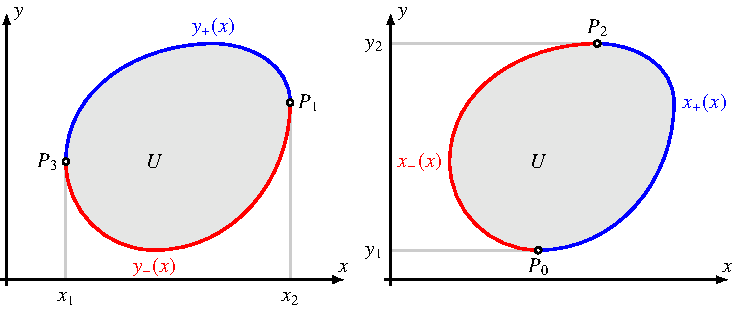
\includegraphics{chapters/040-green/images/greenbeweis.pdf}
\caption{Parametrisierung des Randes des Gebietes $U$ für den
Beweis des klassischen Satzes von Green.
\label{buch:green:green:fig:greenbeweis}}
\end{figure}
%

\begin{satz}[Green]
Für zwei Funktionen $f(x,y)$ und $f(x,y)$ auf einem Gebiet
$U\subset\mathbb{R}^2$ mit Randkurve $\gamma$, die das Gebiet
im Gegenuhrzeigersinn umlaufen.
Dann gilt
\begin{align*}
\underset{U}{\int\!\!\!\int}
\frac{\partial g}{\partial x}(x,y)
-
\frac{\partial f}{\partial y}(x,y)
\,dx\,dy
&=
\int_{x_1}^{x^2}
\int_{y_-(x)}^{y_+(x)}
\frac{\partial g}{\partial x}(x,y)
-
\frac{\partial f}{\partial y}(x,y)
\,dy
\,dx
\\
&=
\int_{y_1}^{y_2}
\int_{x_-(y)}^{x_+(y)}
\frac{\partial g}{\partial x}(x,y)
-
\frac{\partial f}{\partial y}(x,y)
\,dx
\,dy
\\
=
\oint_\gamma f(x,y)\,dx + g(x,y)\,dy
&=
\int_a^b f(\gamma(t))\,\dot{x}(t) + g(\gamma(t))\,\dot{y}(t)\,dt.
\end{align*}
\end{satz}

\begin{proof}
Die beiden Terme des Integranden werden unabhängig voneinander
unter Verwendung der verschiedenen Randparametrisierungen
berechnet.
Die Reihenfolge der Integrationen über $x$ bzw.~$y$ kann daher
in den beiden Teilintegralen vertauscht werden:
\begin{align}
I_f
=
\int_{x_1}^{x_2}
\int_{y_-(x)}^{y_+(x)}
\frac{\partial f}{\partial y}(x,y)
\,dy
\,dx
&=
\int_{x_1}^{x_2}
\bigl[
f(x,y)
\bigr]_{y_-(x)}^{y_+(x)}
\,dx
\notag
\\
&=
\int_{x_1}^{x_2}
f(x,y_+(x))
-
f(x,y_-(x))
\,dx
\label{buch:green:green:proof:eqn:xparam}
\\
I_g
=
\int_{y_1}^{y_2}
\int_{x_-(y)}^{x_+(y)}
\frac{\partial g}{\partial x}(x,y)
\,dx
\,dy
&=
\int_{y_1}^{y_2}
\bigl[
g(x,y)
\bigr]_{x_-(y)}^{x_+(y)}
\,dy
\notag
\\
&=
\int_{y_1}^{y_2}
g(x_+(y),y)
-
g(x_-(y),y)
\,dy.
\label{buch:green:green:proof:eqn:yparam}
\end{align}
Zusammen ist das Doppelintegral $-I_f+I_g$.
Dieses Integral lässt sich jetzt nach 
\eqref{buch:green:green:proof:eqn:xparam}
und
\eqref{buch:green:green:proof:eqn:yparam}
durch Randintegrale berechnen:
\begin{align*}
-I_f+I_g
&=
\int_{x_1}^{x_2}
f(x,y_-(x))
\,dx
+
\int_{y_1}^{y^2}
g(x_+(y),y)
\,dy
\\
&\qquad
+
\int_{x_2}^{x_1}
f(x,y_+(x))
\,dx
+
\int_{y_2}^{y_1}
g(x_-(y),y)
\,dy.
\intertext{Das Integral lässt sich aufteilen in Integrale, die sich
alle mit dem Parameter $x$ schreiben lassen.
Damit dies möglich wird, müssen wir es in vier Teile}
&=
\phantom{+}
\int_{x_+(y_1)}^{x_2}
f(x,y_-(x))
+
g(x,y_-(x))\,y_-'(x)\,dx
\\
&\phantom{=}
+
\int_{x_2}^{x_+(y_2)}
f(x,y_+(x))
+
g(x,y_+(x))\,y_+(x)\, dx
\\
&\phantom{=}
+
\int_{x_-(y_2)}^{x_1}
f(x,y_+(x))
+
g(x,y_+(x))\,y_+'(x)\,dx
\\
&\phantom{=}
+
\int_{x_1}^{x_-(y_1)}
f(x,y_-(x))
+
g(x,y_-(x))\, y_-'(x) \,dx
\intertext{zwischen den hervorgehobenen Punkten
$(x_-(y_1),y_1)$, $(x_2,y_+(x_2))$, $(x_+(y_2),y_2)$ und
$(x_1,y_+(x_1))$
zerlegen.
In allen vier Integralen hat der Integrand die gleiche Form.
In einer beliebigen Parametrisierung
$\gamma\colon [a,b]\to\mathbb{R}^2: t\mapsto(x(t),y(t))$
der Randkurve wird das Integral
zu}
&=
\int_a^b
f(x(t),y(t))\,\dot{x}(t) 
+
g(x(t),y(t))\,\dot{y}(t) 
\,dt
\\
&=
\oint_\gamma f(x,y)\,dx + g(x,y)\,dy.
\end{align*}
Damit ist der Satz von Green bewiesen.
\end{proof}

%
% Der Satz von Green als Spezialfall des Satzes von Stokes
%
\subsection{Der Satz von Green als Spezialfall des Satzes von Stokes}
Die Motivation für den Satz von Green war der Zusammenhang zwischen
dem Integral einer 2-Form auf einer zweidimensionalen Mannigfaltigkeit
mit Rand und dem Integral einer 1-Form.
Dieser Satz gilt aber nicht nur auf einer 2-dimensionalen Mannigfaltigkeit,
sondern kann für beliebige 2-dimensionale Mannigfaltigkeiten, die in
eine $n$-dimensionale Mannigfaltigkeit eingebettet sind.

\begin{satz}[Stokes]
Sie $\alpha$ eine 1-Form auf der $n$-dimensionalen Mannigfaltigkeit $M$.
Sie $S$ eine zweidimensionale Mannigfaltigkeit mit Rand und
$f\colon S\to M$ eine differenzierbare Einbettung von $S$ in $M$.
Dann ist $f^*\alpha$ eine differenzierbare 1-Form auf $S$ und
$df^*\alpha=f^*d\alpha$.
Schreibt man $\omega=f^*\alpha$,
dann gilt
\[
\int_S d\omega
=
\int_{\partial S}\omega.
\]
\end{satz}

Der Satz von Green ist der Spezialfall $M=\mathbb{R}^2$ und $S=U$.

